\graphicspath{{content/chapters/4_specification/figures/}}
\chapter{Specification}
\label{chp:specification}

This chapter outlines the core setup for the project. It begins by examining the dataset’s structure and characteristics, which influence how data is preprocessed and formatted for input to the model. This is followed by a summary of the system-level requirements, including the development environment, training hardware, and memory constraints. Together, these define the context for the design and implementation decisions presented in subsequent chapters.

\section{Dataset Exploration}
\label{sec:dataset_exploration}

A key aspect of defining the system specifications is understanding the dataset used. This project employs an open-source dataset titled \textit{“Noisy speech database for training speech enhancement algorithms and TTS models”}, made available by the University of Edinburgh through its \textit{DataShare} repository~\cite{edinburghdataset}. The dataset is released under the Creative Commons Attribution 4.0 International License~\cite{ccby4}.

\url{https://datashare.ed.ac.uk/handle/10283/2791}

\begin{figure}[H]
    \centering
    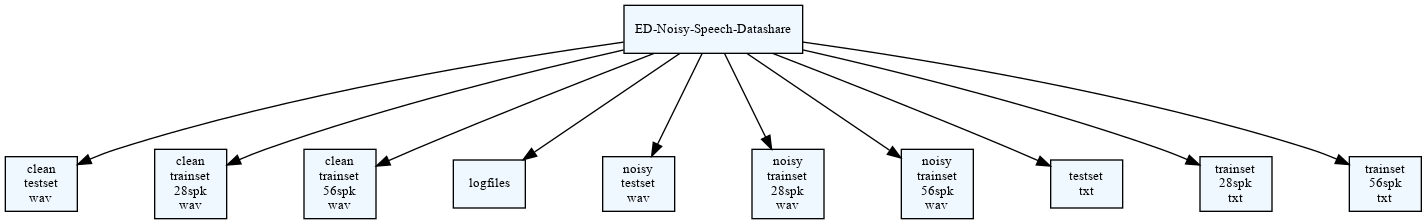
\includegraphics[width=1.0\textwidth]{dataset_structure.png}
    \caption{Dataset Tree Structure}
    \label{fig:dataset_structure}
\end{figure}

As shown in Figure~\ref{fig:dataset_structure}, the dataset is organized into three main subsets: a test set, a 28-speaker training set, and a 56-speaker training set. Each subset includes folders for transcripts, clean speech, and noisy speech. Files are aligned by index across these folders, ensuring parallelism between clean and noisy samples. However, the file numbering is not continuous, with gaps in the sequence.

\begin{figure}[H]
    \centering
    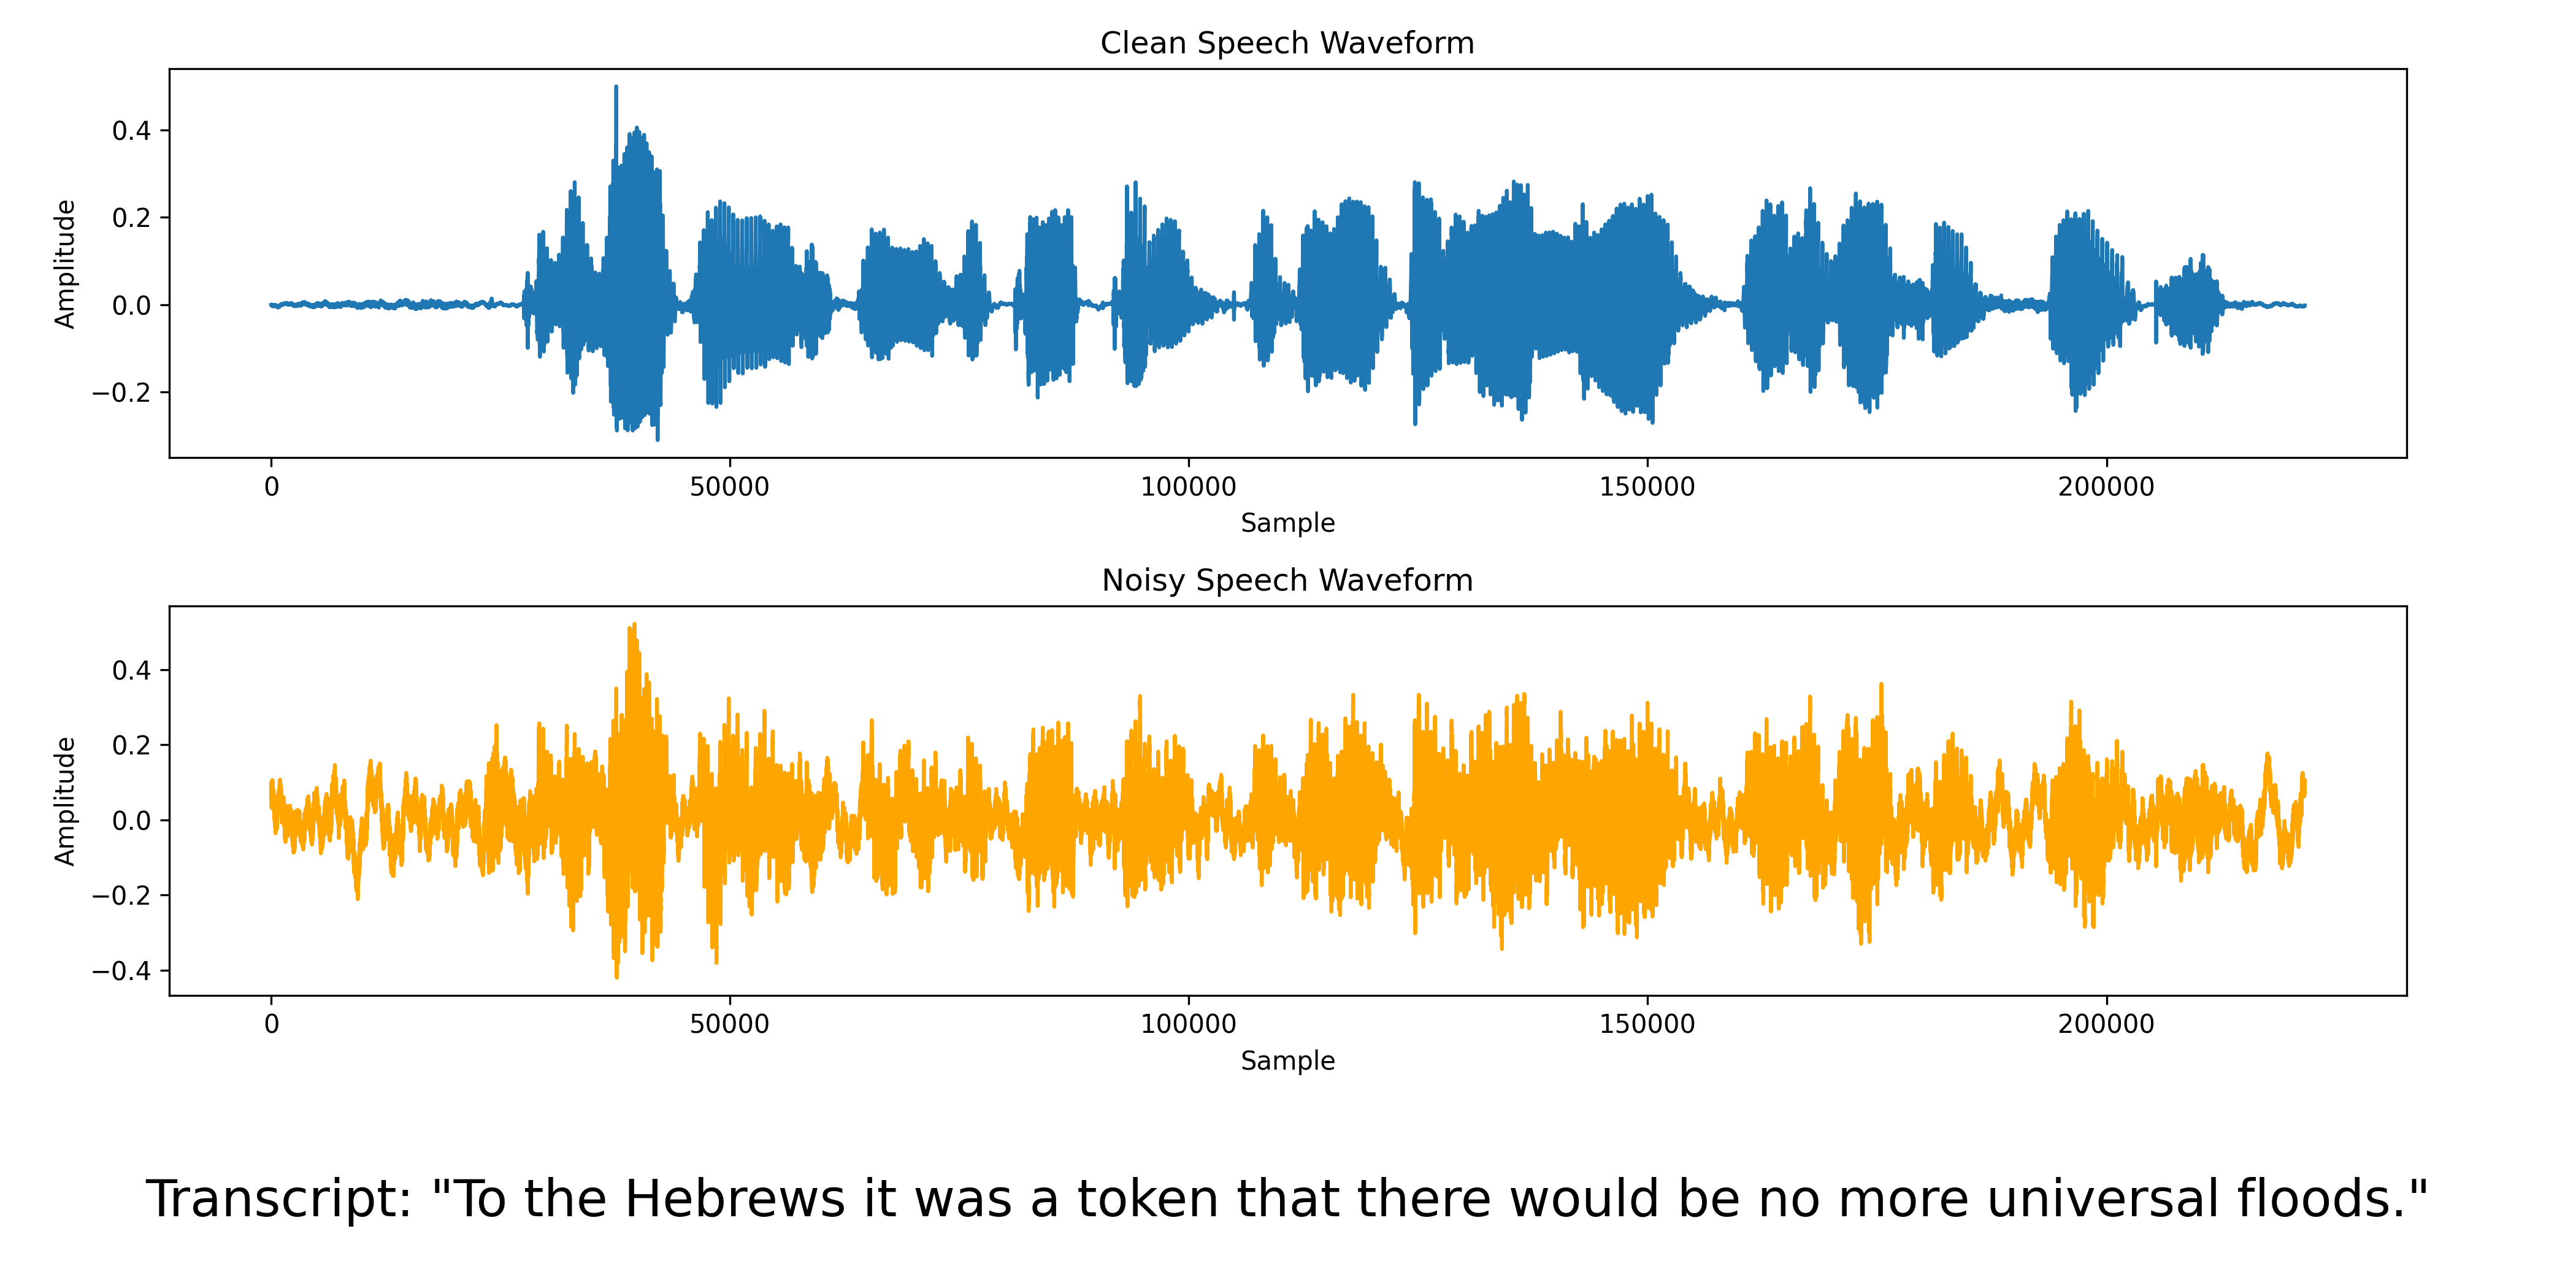
\includegraphics[width=0.8\textwidth]{sample_waveform_and_transcript.png}
    \caption{Example of a Clean, Noisy Speech Sample and its Transcript}
    \label{fig:sample_waveform_and_transcript}
\end{figure}

All audio files are in \texttt{.wav} format and sampled at 48~kHz. Clip lengths vary, which significantly impacts how data is batched and fed into the model. The dataset contains no corrupted files, and the total download size was approximately 15~GB.

\section{System Requirements}
\label{sec:system_requirements}

Given the computational demands of training neural networks, this project was developed and executed remotely on the University of Malta’s Interfacing Lab servers, accessed via \gls{ssh}. These machines are equipped with NVIDIA GeForce RTX 3060 GPUs, which are suitable for deep learning workloads. However, GPU memory limitations required careful control of training parameters, including batch size, model depth, and the number of epochs.

The development environment was based on \gls{vscode}, with assistance from GitHub Copilot for improved coding efficiency. Early experiments and module testing were conducted in Jupyter notebooks, which were later consolidated into a single modular Python application. This modular structure allows for separation of data preprocessing, model training, evaluation, and inference, improving maintainability and extensibility.

The final output of the system is a trained model checkpoint, which can be used for inference on new audio data. The model is compatible with industry-standard frameworks such as TensorFlow and PyTorch and is designed to be portable across machines. This enables future deployment on embedded boards or other constrained platforms for real-time speech enhancement.

